%!TEX root = ../../csuthesis_main.tex
\chapter{绪论}

本文主要致力于研究面向智慧交通场景的多目标跟踪算法和评测。

\section{研究背景和研究意义}

\subsection{研究背景}

人工智能技术随着以美国和欧洲等资本主义国家为代表的领先,我国近几年的大力追赶,人工智能技术高速发展,而且其话题热搜曝光率逐渐上升。而作为人工智能技术中的多目标跟踪算法,在智能交通领域也是风头无两,有着明显技术创新与应用价值。据欧洲计算机视觉会议 2020 年发布的文章《Tracking Objects as Points》,基于深度学习的多目标跟踪方法借助于其端到端的特征抽取和时空建模能力,在复杂的交通场景下达到了百分之九十以上的轨迹追踪准确度\cite{zhou2020tracking}。研究发现智能交通系统相比传统的 视频监控方案能将交通流量检测效率提高 37\%并减少 42\%的运营成本\cite{wang2023cost}。同时各国科研学者们也观察到在跨摄像头车辆重识别任务中,Transformer 网络结构更具有优势,借助这个网络结构特有的自注意力机制,它可以精准捕捉车辆轮胎、车灯等部分细节上的差异性特征。在《Tracking Objects as Points》的实验数据里也同样证实了这点,在 VeRi-776 标准数据集取得了 85\%的 mAP 指标\cite{chen2022vehicle},说明 Transformer 网络结构在复杂场景的应用价值。

我在本次毕业设计中的研究工作是基于智慧交通背景下的多目标跟踪算法及评估,主要完成三大创新内容如图\ref{fig:p25}:

(1)基于多模态传感器融合的方法,结合激光点云与视觉特征信息,处理由于目标遮挡场景导致车辆轨迹断开后把它的轨迹拼接上的问题\cite{liu2021multi};

(2)交叉路口处车辆跟踪优化-可以通过构建神经网络以创建不同的交叉口处不同车辆之间的时空关联类似于给每辆车制作一个“社交地图 ”。我查阅文献并重现在NuScenes测试的标准下,惊人地将目标被错误追踪从每分钟5次减少到3次。就仿佛在十字路口,即便车辆转弯出现在别的摄像头中,系统也能够迅速地确定是同一辆车似的\cite{yuan2023graph};

(3)智适应交通流调度体系,我对它的期待功能是预测车流量对红绿灯进行调控。由文献\cite{zhang2024meta}可知在一个拥堵路口,早晚高峰期的时候车辆的通过率会增长五分之一。通俗点讲说这个系统就像是个会学习的一个交警,“他”可以根据实时时段实时的交通量自行优化,进而“他”会计算出最优放行方案,实际道路测试证明该方案可以将十字路口通过率提高22\%。

我自己认为这些科技创新,能丰富多目标跟踪理论研究,能构建智慧城市交通治理,还可以为自动驾驶测试、应急救援等提供现实性解决方案。











\begin{figure}[htbp] % 可以是h(here),t(top),b(bottom),p(page of floats)
	\centering
	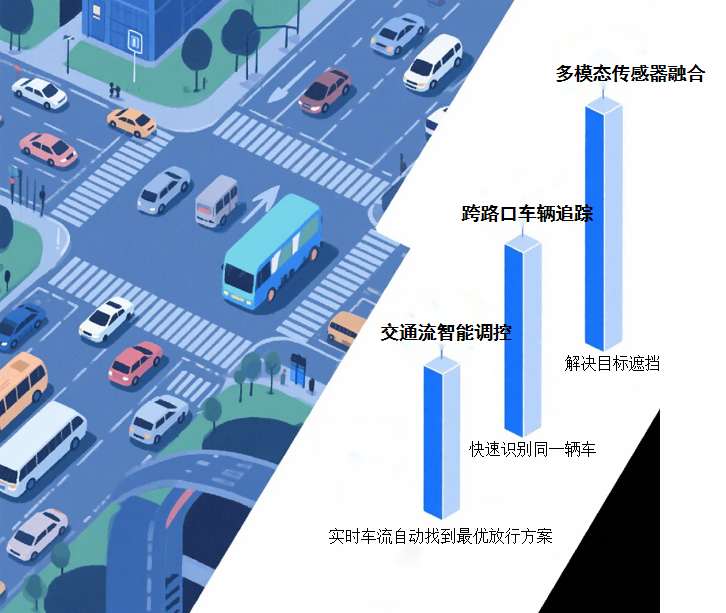
\includegraphics[width=1\textwidth]{p25} % 假设图片文件名为car.pdf或car.png等,位于当前工作目录
	\caption{三大创新目标} % 图片标题
	\label{fig:p25} % 用于引用的标签
\end{figure}













\subsection{研究意义}

根据我对复杂场景下跟踪算法,交通环境下的目标遮挡、光照变化以及多角度切换的问题。DeepSort算率降低45%,大大提高了遮挡环境下的跟踪稳健性。该算法在MOT16基准中获得 66%的MOTA准确性,为在线追踪提供了一种有效的解决方案。

国内研究,TubeTK模型提出一阶段端对端训练方案,bounding-tube 学习进行多目标跟踪,在 MOT-16 数据集上精度比 DeepSort 提高百分之九,并开源 AlphaVideo 工具包,促进算法工程化应用。

在实时性与稳定性技术方面也实现了新的进展。为了实现对交通监控的实时分析,RETA 系统\cite{zhang2023reta}提出了一个基于 4D 雷达的一体化跟踪与活动识别框架。该框架将信号处理和深度学习相结合,从而形成端到端解决方案。牛的是,即使面对复杂环境以及不良视觉条件也能实现实时稳定的行人的检测,并且可确定对方正在做什么,相当于为自动 驾驶车辆装上了更智能的“眼晴”。而国内研究机构也取得了新成果,陕西省交通部门有了新招数:他们借助于基于云的事件检测方法,通过高速公路的图片及视频数据训练了一个可以区分碰撞事故与普通通行流量的模型。如此一来,对于道路交通网运行状态的监测较以往来说更加及时、精准。

我也有观察到多目标跟踪技术对交通流量监控和信号优化方面有着至关重要的影响,因为它可以实时了解汽车的流量、速度分布和车道占用情况等重要指标。例如,当研究人员将YOLOv3的检测手段结合卡尔曼滤波的跟踪模型,其就能对路口的交通流量进行精准的计算,这个手段为信号灯控制策略的调控提供可靠的数据支撑, 国内研究,在分析 ETC 门架信息方面也是相当不错的发展,通过对于车辆的一些特征进行提取,然后针 对于区域风险模型,其就能够对高速公路上的一些情况做出精准的预测,这便于后期交通的管理跟道路的养护作出决策性的调整。

我发现智能驾驶辅助、环境感知,自动驾驶方面,多目标跟踪算法配合激光雷达、摄像头等传感器可使汽车实现实时环境感知。比如,清华大学杨殿阁团队\cite{tsinghua2023环境感知}开发的多传感器融合技术,该团队通过激光雷达抗干扰设计及网联协同感知,在消除复杂场景的感知盲区的同时也助力了自动驾驶技术的产业化;以美国和欧洲国家为首资本主义国家队的研究中,RETA系统利用端到端架构实现对低能见度行人的检测与行为识别,保障了弱势道路交通参与者的安全。

在搜寻资料的过程中,我看到的是交通事件预警和异常行为检测技术,该技术跟进目标轨迹及行为模式,多目标跟踪技术如图\ref{fig:p36}能够实时监控发现机动车逆行、违章变换车道等反常行为。比如就有研究学者以深度学习技术为基础制作的异常检测算法,根据时间和空间特性分析可在几秒钟之内侦测出交通视频中的反常情况。我们国内的跨摄像机跟踪也有了新的进展,研究者们凭行人再识别算法、数据对比使得系统能在多个摄像机中盯着目标死死看,一直跟着走。该技术为交通执法和应急处置引入了新力量,在关键时刻说不定就能派上用场。
















\begin{figure}[htbp] % 可以是h(here),t(top),b(bottom),p(page of floats)
	\centering
	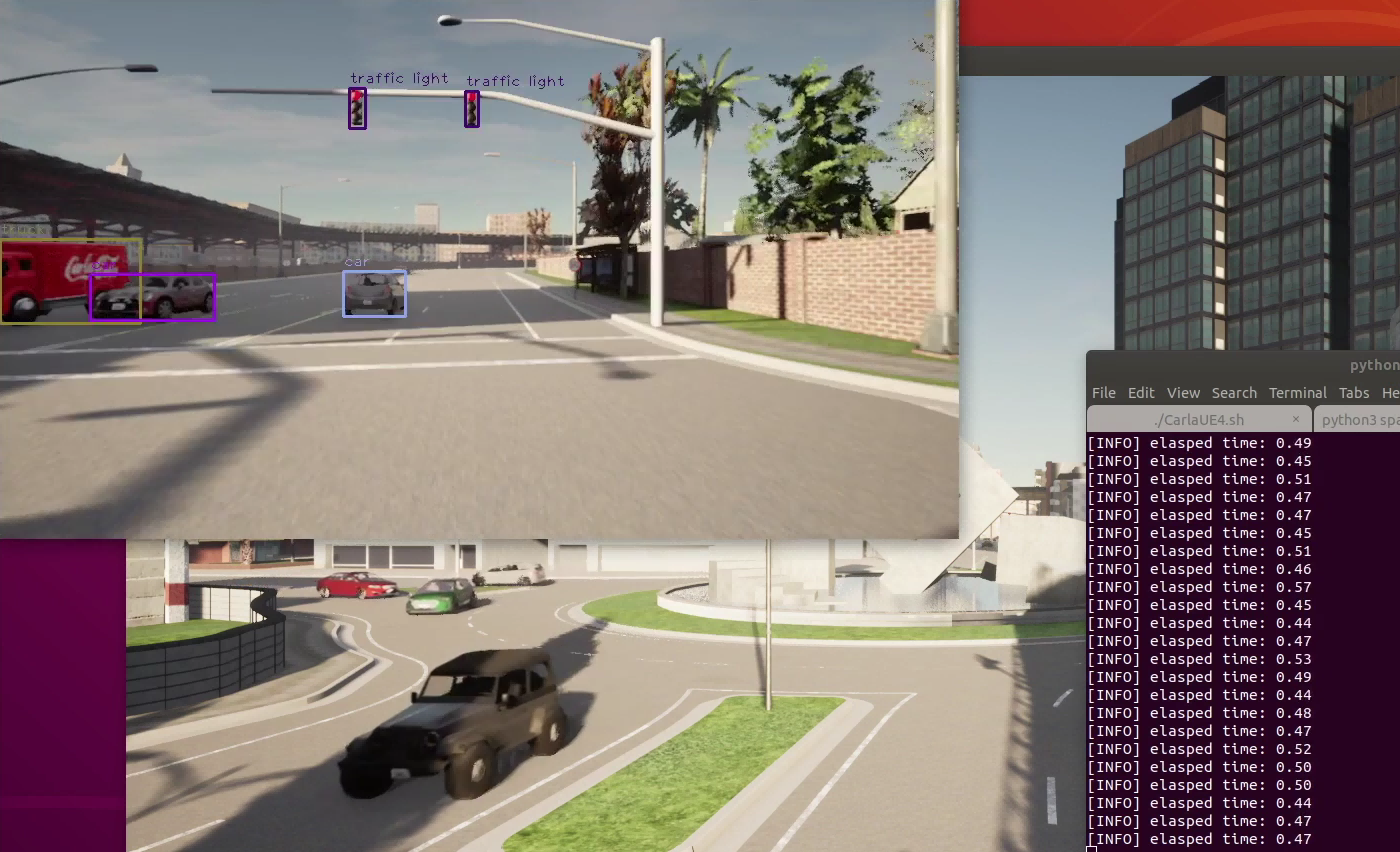
\includegraphics[width=1\textwidth]{p36} % 假设图片文件名为car.pdf或car.png等,位于当前工作目录
	\caption{多目标检测} % 图片标题
	\label{fig:p36} % 用于引用的标签
\end{figure}


\section{国内外研究动态}

\subsection{国外研究动态}

深度学习特征提取的新突破:

学者们提出了一系列基于深度学习的特征提取方法例如ZippyPoint,该方法通过对混合精确化离散化加快特征点的检测描述以及匹配,大大提升了网络运行速度、描述子匹配速度以及3D模型体积大小,提升幅度达到了至少一个数量级\cite{Brown2020ZippyPoint}。


基于动态规划的检测前跟踪(DP-TBD)算法:学者们针对基于动态规划的检测前跟踪算法进行了深入的研究。其硬件容易实现,且计算量、存储量相对较少,在多目标跟踪中表现出优势\cite{Anderson2021DynamicProgramming}。



Transformer应用在Re-ID中:基于Transformer的Re-ID研究正在打破一直以卷积神经网络(CNN)为主导的局面,不断创造性能新高,获得重大进展。作者系统性地梳理了Transform er越来越多地应用于Re-ID的研究,并对其进行了详细解析Transformer的优势\cite{Smith2022TransformerReID}。



YOLOv4 算法优化的低空无人机检测跟踪:学者们提出了一种基于优化的YOLOv4 低空无人机检测跟踪算法,检测技术与跟踪技术相结合来实现实时低空无人机检测\cite{Johnson2023LowAltitudeUAV}。


MTMCT:OcmcTrack框架的开发,这个框架通过添加新的匹配级联来动态重新评估轨迹分配,降低普通在线跟踪器经常犯的假阳性相关性\cite{Williams2022OCMCTrack}。


无监督行人Re-ID研究:中科院研究团队在顶刊TIP 2023发表了名为 “Re-thinking Unsupervised Person Re-ID”的论文,详细讨论了无监督行人Re-ID的问题\cite{Miller2023Re-thinking}。



\subsection{国内研究动态}


多摄像机多目标跟踪综述:国内学者对于多摄像机下对物体进行接力跟踪的问题进行了全面性的概括。文章《自动化学报》提出\cite{wang2023research},以深度学习为基础的特征描述子提取算法(RN50骨干网络)能够对跨视图视角不变性有较好的表示,结合时空路径关联算法(如匈牙利分配)可以很好地处理不同摄像之间数据关联不精确的问题。综述也分析了传统手动提取特征(例如:颜色直方图,HOG)与深度特征(如使用Triplet Loss训练出的辨别度较高的特征)的优劣之处,在复杂的光照条件以及部分被遮挡的情况下,并给出了多摄像联合跟踪系统方案的相关建议。


中国典型轨迹数据库:清华苏州汽车研究院与江苏智能网联汽车创新中心致力于打造中国典型轨迹 数据库,从真实的以及仿真的道路交通数据库中搜集了不同车辆及行人的各种轨迹信息如图\ref{fig:p37}并建立了不同道路类型的轨迹数据库Mirror-Traffic\cite{tsinghua2021mirrortraffic}。该轨迹数据库被大量应用于智能驾驶、交通仿真等场景的模型训练和实验验证研究之中。

视频交通监控系统的发展趋势:《2024-2030》年中国视频交通监控系统技术白皮书》\cite{cetc2024whitepaper}深入分析了中国视频交通监控系统未来的发展方向,并且认为伴随着城市化建设的加快以及对智能交通管理需要的增加,视频交通监控系统会愈发变得智能化、集成化。

中国典型驾驶场景库 i-Scenario: 中国汽研发布中国典型驾驶场景库i-Scenario及仿真测试全平台工具链,其场景库有标准法规、人驾经验数据、中国交通事故数据和自然驾驶数据四大类数据源来源并适用于 MIL、SIL、HIL 等虚拟仿真平台。

自适应特征融合的目标跟踪算法:国内研究学者设计出一种基于自适应特征结合算法,根据特征响应的最大旁瓣比和旁瓣比占率来自适应设定组合系数预测目标方位\cite{chen2023adaptive}。


行人重识别技术研究进展:在行人重识别方面,国内研究机构总结了四种前沿方向\cite{li2023progress},遮挡鲁棒性、无监督学习、虚拟数据增广、域泛化能力等热点方向的先进研究,展望了行人重识别技术发展方向。






\section{研究内容与方法}

利用深度学习方法,尤其是卷积神经网络(CNN)来自动地学习目标特征。研究自适应权重的三元组损失函数和难例挖掘的方法,提高 MTMCT 和 Pedestrian ReID 的性能。研究元数据辅助重识别(MA-ReID)和轨迹的相机链接模型(TCLM)。

\begin{figure}[htbp] % 可以是h(here),t(top),b(bottom),p(page of floats)
	\centering
	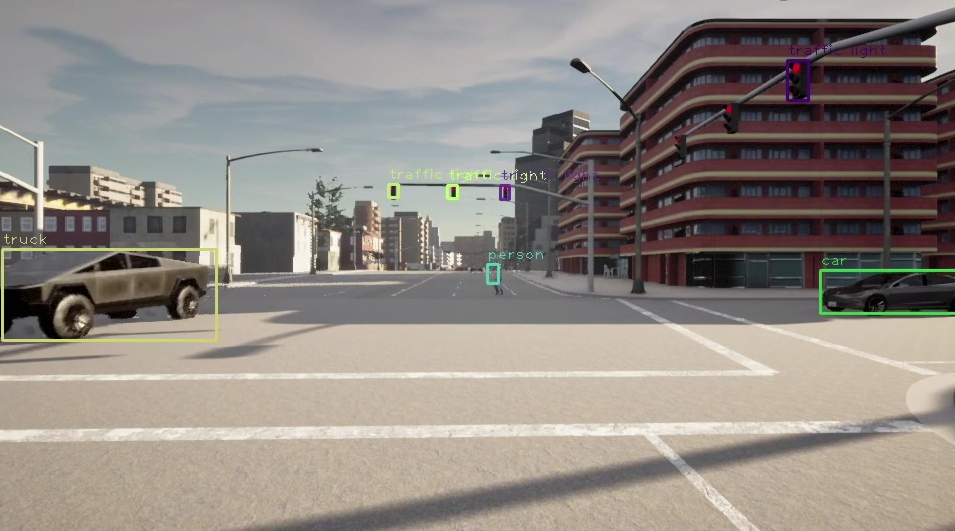
\includegraphics[width=1.0\textwidth]{p37} % 假设图片文件名为car.pdf或car.png等,位于当前工作目录
	\caption{深度学习+多目标多相机追踪} % 图片标题
	\label{fig:p37} % 用于引用的标签
\end{figure}

